\chapter{码中一窥C++}

凡是语言,都一定有着自己的规则。而不同于英语、汉语这种自然语言,作为计算机所能识别的语言,它是需要在严格约束下避免二义性的,所以说我们将学到的C++语言,是一门语法规则非常严格,但又“灵活多变”的语言。

所谓非常严格,是指C++中不允许出现歧义,这种没有歧义的文法是经过严格的文法规则的限制、和一些约定来约束的。所以,如果在你的代码中出现了自己都会觉得有歧义的地方,往往就是程序中容易出错的地方。

而所谓灵活多变,就是指在掌握C++严格的语法之后,可以写出无穷无尽充满创意的程序。从黑框(控制台程序),到带有图形界面(GUI)的程序,再到游戏,都可以利用C++的语法加上你脑中的算法搞定!而所有的这些灵活多变的内容,都是在严格的文法约束下实现的。所以说C++语言,是一门语法规则非常严格,但又灵活多变的语言!

C++是一门高级语言,所谓高级语言正如你们在前面章节中看到的,是不同于机器语言、汇编语言;能更加贴近人类思维的一门语言。C++是在C语言的基础上,增加了例如面向对象编程等诸多特性的程序设计语言。在程序设计竞赛中被广泛采用。

非常不严格地讲:我们常常所说的“C++”,包含了这门语言和一系列的工具。语言顾名思义就不多阐述。而工具实际上包含了很多内容:

我们将C++语言所编写的代码叫做“源代码”。而源代码是不能直接被计算机执行的(回想我们在上一章中讲述的内容)。而是应该利用编译程序,将源代码编译成计算机能够识别的机器代码然后再执行。而执行编译工作的工具就叫做“编译器”。

除此之外,仅仅有C++语言,我们连基本的功能(例如屏幕输出)都实现不了。即便是高级语言,想要与硬件设备交互,一般都需要直接编写一定的机器语言或者汇编语言,所以才能让我们的程序操作硬件:屏幕打印、屏幕输入、文件操作等等。而我们想要通过一己之力实现这些最底层的操作是很困难的。好在C++提供了一组可以被调用的工具。这些工具其实就是别人写好的代码,通过C++语法能够接受的形式所调用,最终辅助我们完成底层调用的功能,让我们的精力能够集中在更重要的算法设计上而不是千篇一律的与底层的通讯上。我们称这种“别人的代码”叫做“库”。就如同仓库一样,我们可以调用仓库中的内容来实现我们的意图。

那么我们的程序是怎么与别人的程序产生关联的呢?这有很多种情况,我只讲述最常见的一种:静态链接。我们的程序在调用库的时候,编译器可以仅仅在相应的位置上做个标记,表明这里的程序是调用了库而不是我自己的。这么做的好处就是可以充分地提高编译效率。因为库中的代码往往经过严格的编写、测试,基本能保证没有问题,所以我们只需要保存该库编译完毕的状态,没有必要在编译自己的程序时还要将别人的库再编译一遍。我们只需要编译自己的程序就可以了。所以我们的程序与库之间是并列关系,而不是包含关系。但是想要让自己的程序能够变成可执行程序,仅仅是这种“做标记”的方法是不可接受的。因为你所需要的库文件在你的电脑上会有,但并不意味着别人的电脑上也会有。再加上可执行程序的复杂原理,我们必须将这些静态库与我们的程序绑定在一起。而将编译完的“目标代码(Object Code)”与库文件链接形成“可执行文件”的工具叫做“链接器”。

也就是说,C++程序设计流程是:
\begin{quote}
	\begin{enumerate}
		\item 编写代码
		\item 编译成目标代码
		\item 链接成可执行文件
	\end{enumerate}
\end{quote}


一般来说,想要实现上面的流程,需要利用操作系统提供的黑框(Linux下的终端、Windows下的控制台),再加上一大堆非常复杂的命令才能实现。编译命令甚至有可能比源代码还要复杂。如果需要对自己的代码进行调试,那可是更加麻烦。所以聪明人们就为懒人发明了又一件工具:集成开发环境(Integrated Development Environment,IDE)。所谓开发环境,可以将其看作是写代码的一个工具。我们可以在这个开发环境中编写代码、代码着色、自动排查错误等。所谓“集成”就是指将“编译器”、“连接器”都集中在IDE中。程序员可以简简单单地点击按钮,就可以实现整套编译链接运行调试等功能。

在ACM/ICPC的比赛中,通常使用的编译器是GCC(GNU Complier Collection)。GCC是一个支持很多种语言的开源的编译器的集合。它可以安装在Windows(不推荐)和Linux等多种操作系统上。而在比赛中普遍使用的是安装了Linux操作系统和GCC编译器的开发环境,并且配置了某些IDE来让学生进行开发。

关于IDE:对于Windows来说,我门推荐使用Dev-C++。对于Linux,我们推荐使用Code-Blocks。

本章的行文基于“CART”步骤,即(C)ode, (A)nalyze, (R)esult, (T)ry。四步。

Code是指展示代码,Analyze是针对代码分析其中的语法元素,Result是根据程序的运行结果来分析程序的逻辑,Try则是举一反三,完成与该代码相关的另一段代码的编写。

\section{Helloworld++}
其实吧,作为一名编程初学者,第一个编写的程序应该就是传说中的“Helloworld”。这个程序意图就是在屏幕上简简单单地打印出一个“Helloworld”的文字。目的是为了表示当前的开发环境没啥问题,可以继续工作了。

但是我觉得一个Helloworld太简单了,各种书籍都把这个例子用烂了,那我在这里就用一个稍微复杂的例子来实现这个“Helloworld”吧!

\subsection{Code}
\lstinputlisting[language=C++,caption=Helloworld++,label=code:helloworld++]{codes/1-1/1-1.cpp}

\subsection{Analyze}
代码\ref{code:helloworld++}是加强版的Helloworld,所以我管它叫做Helloworld++。代码首先通过提示依次输入你的姓名和性别,再根据不同的性别输出不同的“问候语”。对它的部分解读如下:
\begin{quote}
\showremarks
\end{quote}

我们再来逐行精读这段代码。

首先,代码\ref{code:helloworld++}的前两行中使用了“\#include<xxxxx>”。这部分内容叫做“预编译指令\footnote{也叫做预处理指令。}”。所谓预编译,就是指在编译之前要“告诉”编译器的“话”。编译器收到这些指令之后就会按照指令上的内容提前进行一些预处理。

在C++中常见的预处理指令主要有“\#include”、“\#define”等。当然还有一些诸如“\#ifndef”等在本书中不是很常用的预处理指令。

“\#include xxx”用来表明该段程序编译前应该包含哪些其他文件。由于操作系统会将一些常用的操作封装成函数库,并写在某些自带的文件中,所以当我们使用这些函数库的时候,一般都需要通过该命令将其包含。命令中的xxx则是用“<>”或者双引号括起来的文件名。用“<xxx>”则表示这个文件在系统的搜索路径下保存,一般是系统库。而用双引号扩起来的则表示这个文件跟当前程序代码文件存放在同一个文件夹。

而“\#define A B”则是表示强行将B替换成A。也就是说在以后的代码中凡是出现过“B”的地方都将会无条件地被替换成“A”。在C语言\footnote{C++的前身,C++就是对C语言扩展而成的语言}时代,常常用这种方法来避免一些硬编码\footnote{即“直接将常数值分布在程序的各处”,这种硬编码导致的程序冗余性会让代码修改起来非常困难。}。例如有一个运算式频繁使用了PI=3.14这个数值。但是突然想要让PI=3.1415。这时候需要把所有的3.14替换成3.1415。但如果很早之前我们的程序就是用PI来表示这个值,在此时也就只需要将“\#define PI 3.14”改成“\#define PI 3.1415”即可。

由于“\#define”是在“编译前”执行,所以它带来的开销不会在程序运行时体现出来,而且还能进行很多技巧性的操作。但是由于这种“技巧性”的操作稍有不慎就可能产生很麻烦的后果,所以不建议初学者滥用这种方法。而它所提供的功能可以通过类似但更加安全的方法实现。

代码\ref{code:helloworld++}的第三行用来“使用命名空间”。所谓命名空间,是一种C++对多文件多函数的组织工具。我们常常把功能相近的函数库放在一个模块中,为这个模块可以取一个好记的名字。当以后使用这些函数库时,就可以使用using namespace xxx; 这样的语句来使用。

在代码下面的诸如“cin”、“cout”、“endl”等内容,以及以后大家将会接触到的一些函数库都需要“std”命名空间,大家记住在每次编写代码时都写上这一句就好了。有关命名空间的详细主题已经超过本书“速成”的要旨,就不多介绍了。

程序的第五行是定义了主函数。所谓函数,暂时可以理解为对一组操作的包装\footnote{术语叫做“封装”}。而主函数则是整个程序的入口。可执行文件被打开后,操作系统将会从主函数开始依次执行。在主函数中又调用了各种各样其他的程序,以此来完成整个运行逻辑。

之所以称之为主函数是因为它的结构。int main()表明这是一个返回int类型\footnote{什么叫做“返回int类型”,我们稍后再谈}的函数,而函数名“main”则表明了这个函数是一个主函数。后面紧跟着一个大括号。主函数内部的东西都写在了这个大括号中。

一般来说,大括号表示一段语句,而其中的语句隶属于这个大括号,所以在大括号中的代码应该比外面的代码多缩进一截。这么做对编译器没有任何影响,只是为了让代码层次感明确、易读。所以希望大家都遵守这个惯例!

在大括号中的内容就是系统会执行的代码。第七行的内容称为注释。注释就是一种会自动被编译器所屏蔽的“非代码”。注释能够辅助程序员解释代码功能,增加代码可读性。同时由于“被注释后会被编译器忽略”的特性,使得注释可以用来“临时屏蔽”一些代码。

在C++中添加注释有两种方法。一种是行注释:“//”——两条正斜杠后面的内容都是注释。还有一种是块注释:“/*”到“*/”中间的所有内容,无论经过多少行,都会被看做是注释。正如同代码的第7、10、13行。

在代码的第8行,声明了一个常量。此处的常量与数学意义上的常量非常类似。常量的定义通常由两部分。

一部分是定义部分,形如“const int trunk\_size”。其中“const”是定义常量的关键字\footnote{一般与“保留字”等价。他们是一种特殊的单词,这些单词不能作为常量、变量名等用户自定义的内容。因为它们本身已经被C++编译器赋予了神圣的意义。}。“int”表示这个常量的类型是“整型”。关于数据类型将会在后面介绍。“trunk\_size”就是变量名咯,是这个常量的名字。

另一部分是赋值\footnote{赋值就如同数学中的等式,将等号右边的值赋予等号左边的“名字”,从此这个“名字”将会与该值绑定}部分,形如“trunk\_size=100”。这部分内容就是指令常量“trunk\_size”等于常量值“100”。(跟我们学过的数学完全一样是吧!)

既然名叫常量,则就说明这个量一经定义不许再在程序中改变。所以常量的定义部分和赋值部分是合在一起的,形如第8行代码。此之于“变量”来说是略有不同的,我们将稍后再说。

在第11行和14、15行有两条非常相似的语句。这就是传说中的变量定义。其实变量定义跟常量定义非常相似,反倒是常量定义麻烦了一些——变量定义不需要const修饰。在11行,定义了变量,并且直接在等号右边赋值。第14行则是先定义变量,再在第15行赋值。

变量定义部分的“char *”表示了这是个“字符指针类型\footnote{指针,即“保存内存地址”的变量,该主题将会在后面谈到}”。“name”和“sex\_str”是变量名。而等号后面的赋值部分,实际上是在进行“在堆中申请一段连续存储空间”的操作。上面这堆文字具体的意义我们后面会详细提到,目前你只需要知道这就是声明变量的一种方法就好了!

在第17,18行,有一种“cout<<xxxx<<endl;”的格式。其中cout是输出流对象。也就是说需要输出的时候就靠它。而在第19行的cin则是代表输入流对象。这两种对象对应着不同的符号进行控制。如果说这种大于号和小于号类似于箭头,则可以将“cout”和“cin”分别看作是屏幕和键盘。数据从箭头起点处流向目标。而且cout和cin必须要写在开头。于是就有了例子中的样式:第17行的“Who are you”作为数据,被传送到了cout这个“屏幕”。然后又将“endl”这个换行符传递给了cout。在第19行则表示将键盘的内容输出到“name”这个变量中。

代码的第17-23行都是在进行输出和输入。而在24行到28行则是一种特殊的结构——选择结构。

所谓选择结构,就是指根据某个条件进行选择。如果这个条件成立则做事情A,如果另一个条件成立则做事情B,以此类推,直到什么都不成立的时候,则做另一个事情。

这五行代码是选择结构中的if语句。形式大约是:
\begin{quote}
if(<事件A>)\{

	\qquad 若A事件成立则执行此块
	
\}else if(<事件B>)\{

	\qquad 若B事件成立则执行此块
	
\}else\{

	\qquad 若都不满足则执行此块
	
\}
\end{quote}

值得注意的是在第24行的“strcmp("boy",sex\_str)”。这是一个系统库“<cstring>”中的函数“strcmp(strA,strB)”。这个函数的功能是比较字符串。若strA与strB的内容完全相等,则它的值等于0。在这个函数调用前的感叹号是“取反”符号,功能就是让1变0、0变1。所以这段代码的逻辑就是:如果sex\_str等于“boy”,则执行第25行。否则执行27行。

在第29行,“return 0”表示这个函数返回“0”。由于这个函数是主函数,则它的返回值将会被操作系统所接收\footnote{有关函数和返回值的相关主题将会在后面介绍}。

至此我们便大致分析了这个“Helloworld++”程序。接下来我们执行以下看看结果!

\subsection{Result}

根据程序逻辑,这段代码执行时要先输入一个名字,然后输入boy或者girl,屏幕则会根据这些不同的输入打印出不同的响应文字。
\\[\intextsep] 
  \begin{minipage}{\textwidth} 
    \centering 
    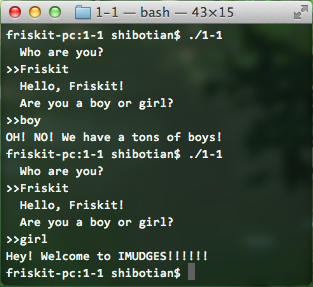
\includegraphics{codes/1-1/result.png}
    \figcaption{Helloworld++} 
    \label{fig:code-1-1-result} 
  \end{minipage} 
\\[\intextsep] 

我们再来分析一下这个程序的运行逻辑。
\begin{quote}
	\begin{description}
		\item[步骤1>>]在程序的1-2行,通过预编译指令,包含了两个函数库文件。
		\item[步骤2>>]在程序的第5行找到程序的入口、主函数。
		\item[步骤3>>]在程序的第8~15行定义了一系列常量和变量。
		\item[步骤4>>]在程序17~18行输出提示信息,让用户输入名字。
		\item[步骤5>>]等待用户输入名字,并将输入内容存储至变量“name”。
		\item[步骤6>>]再提示用户输入性别。
		\item[步骤7>>]等待用户输入性别,是“boy”或者“girl”。并且将输入内容存储至变量sex\_str。
		\item[步骤8>>]判断sex\_str里的内容。
		\item[步骤9>>]如果内容是“boy”则执行第25行的输出。
		\item[步骤10>>]如果内容不是“boy”则执行第27行的输出。
		\item[步骤11>>]主函数返回,程序结束。
	\end{description}
\end{quote}

至此就是这个程序的运行流程。

我们再来小结一下上面的程序所遇到的内容!希望大家在看到这些名词之前能努力回忆一下它们的具体含义。然后再看后面的解释内容!

\begin{description}
	\item[预编译指令]被编译器在编译前执行的命令。包括“\#include”、“\#define”等等。
	\item[命名空间]命名空间是C++用来高效地组织各种代码的方法。通常我们使用的命名空间是“std”。用法是:using namespace std;
	\item[主函数]整个程序运行的入口。它的返回值将会被操作系统所接收,你可以通过返回值告诉操作系统这个程序结束执行时的状态。例如0表示正常,-1表示错误。
	\item[变量]变量就如同数学中的概念一样,是一种可以变化的量。变量就是内存中固定大小的一块存储空间,其大小由其类型决定。变量使用前需要预先定义!
	\item[常量]常量是一种一经定义就不能改变的量,也正是因为这个特性,它必须在定义的时候立刻赋值。将一般不会改变的数存储成常量而不是变量,一来能防止不小心地修改这些值,另一方面能够通过系统的内存管理机制得到优化。
	\item[标准输入输出]即“cout”和“cin”。就是一种用来控制“输出到屏幕”和“从键盘读取”的工具。大于号或者小于号表示输出方向。将“cout”看作是屏幕、将“cin”看作是键盘,将会比较容易加深记忆。
	\item[if语句]它就是一种选择结构的语句。就如同数学中的分段函数一样,根据不同的条件进行不同的操作。大家再回忆一下它的形式。
	\item[语句]语句就是C++程序中的基本组成单位。变量定义可以使一个语句、赋值操作可以是语句、函数调用可以是语句,还有一些程序控制语句(例如if语句等)。总之,我们的程序是由一个个语句组成的。在语句之中可以嵌套其他语句。
	\item[关于分号]一般来说,除了预编译指令以外,我们需要在每一个语句完成之后加上分号。
\end{description}

在这一节中,大家了解到了一个完整的不算大也不算小的C++程序的样子。我们今后所编写的代码也基本都长这个样子,区别就是主函数里头的东西可能更丰富、算法更高深等等。但是这个整体的框架是万变不离其宗的。所以希望大家能够根据上面的例子“改造”出自己的代码来。

\subsection{Try}

在了解完上面的例子,我们可以用类似的代码“创作”出一些自己的程序!

\begin{description}
	\item[Try 1]制作一个程序,在屏幕上输出一行“Hello World!”。
	\item[Try 2]制作一个加法运算器,根据提示分别输入加数和被加数,并且输出两者相加的结果。
	\item[Try 3]制作一个程序:用户输入数字1-7,输出汉语“星期x”,(使用连续的if-else if语句)
\end{description}

\section{使用变量与数据类型}
我们在前面曾经讲过,现在的计算机都是一种“存储计算模型”。“存储”在程序中的体现就是“变量”。变量其实就是在程序运行时用来存储数据的容器。它的物理结构就是内存中的某一块固定大小的区域。尽管都是用“0”、“1”将内存区域填满,但不同类型的变量所占用内存单元的数量会有所不同,也会导致这种类型所表示的数据范围的不同。同时,一般的数据类型还有“有符号”和“无符号”的区别。这是由于计算机利用数据单元中的1位来表示正负,所以即便是能够表示数字的数量相同,但能表示的范围仍有所区别。

在C++中有一些内置的基本数据类型,用户也可以定义自己的数据类型。不同的数据类型以不同的排布方式放置在内存中。数据相同的内存单元,用“不同类型的角度”来看都有不同的取值。常见的基本内置数据类型如下:


\begin{table}
	\begin{center}
		\caption{基本数据类型}
		\label{tab:DataTypes}
		\begin{tabular}{|c|c|c|}
			\hline
				数据类型 & 长度 & 能表示的数据范围\\
			\hline
				char & 1 & $-128 \sim 127$				\\
				bool & 1 & true or false				\\
				short & 2 & $-32768 \sim 32767$			\\
				unsigned short & 2	 & $0 \sim 65535$\\
				int & 4 & $-2147483648 \sim 2147483647$	\\
				unsigned int & 4 & $0 \sim 4294967295$ \\
				long & 8\footnote{} & $-9223372036854775808 \sim 9223372036854775807$	\\
				unsigned long & 8 & $0 \sim 18446744073709551615$ \\
				float & 4 & $-3.4\times10^{-38} \sim 3.4\times10^{38} $ \\
				double & 8 & $-1.7\times10^{-308} \sim 1.7\times10^{308} $\\
			\hline
		\end{tabular}
	\end{center}
\end{table}
\footnotetext{在32位计算机上长度可能为4字节,功能和取值范围与int完全一致}

了解了上述的数据类型之后,让我们来看看这一节的代码吧。

\subsection{Code}

\lstinputlisting[language=C++,caption=数据类型,label=code:DatatypeTest]{codes/1-2/1-2.cpp}

\subsection{Analyze}
首先我们看看上面代码的一部分注解:
\showremarks

上面的程序进行了很多关于数据类型的试验。

在8至13行,分别测试不同的基本数据类型在内存中所占空间的大小。在第16至24行进行了一些数据的“边界”操作。

在第28行,我们尝试输出了int类型变量“int\_number”在内存中的表示。而在第31行又输出了float类型变量“float\_number”在内存中的表示情况。

在33行以后,程序又测试了有关类型转换的内容。

\subsection{Result}
我们再来看看这段程序运行后的输出:
\\[\intextsep] 
  \begin{minipage}{\textwidth} 
    \centering 
    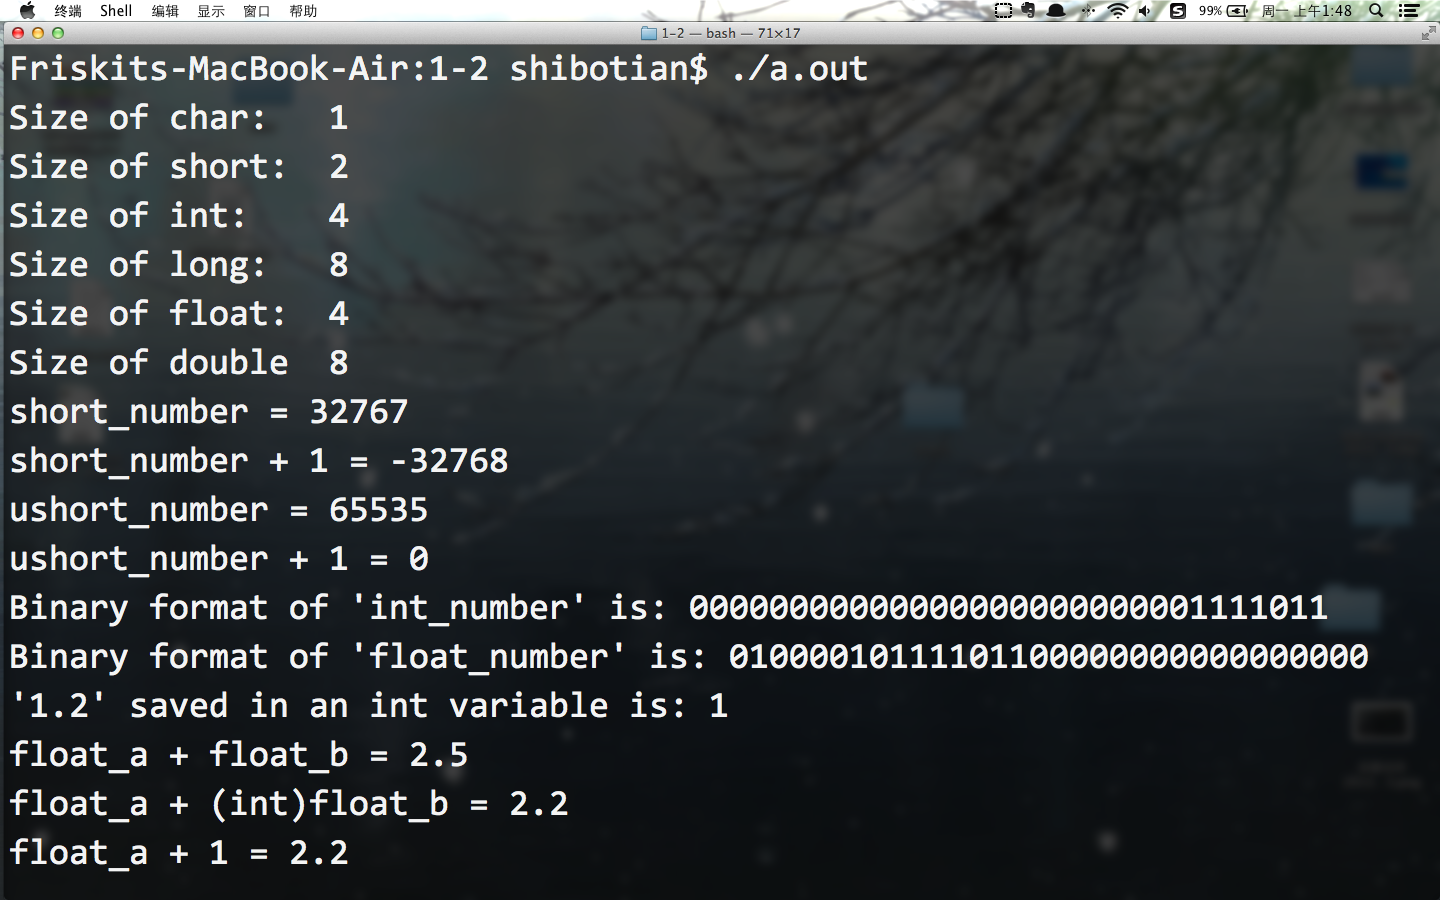
\includegraphics{codes/1-2/result.png}
    \figcaption{数据类型测试} 
    \label{fig:code-1-2-result} 
  \end{minipage} 
\\[\intextsep] 

输出结果首先验证了我们先前讲过的几种基本数据类型不同的占用内存空间大小。然后测试了当数据溢出时导致的问题。

“通常”来说,溢出后是一种“循环”的效果。最大值+1会变成该数据范围内的最小值、最小值-1则会变成数据范围内的最大值。而“unsigned”放置在类型关键字前,用来表示这种关键字是否需要包含正负号。有unsigned修饰,则表示这个类型是无符号的,反之亦然。unsigned关键字只是用来改变数据范围覆盖的窗口,但并不能改变当前变量内表示数据的个数。但当我们的变量只可能表示正数或者负数时,则使用unsigned可以让正数、负数的个数增加一倍。

再到后来,程序输出“ '1.2' saved in an int variable is: 1 ”。此处对应代码的第24和35行。此处我们将一个“float”类型的字面常量\footnote{所谓字面常量就是指“所见即所得”,看到的内容就是常量值,例如int类型字面常量123,例如字符串常量“Helloworld!”。与之对应的另一种常量成为“符号常量”,就是例如“PI”这样的有名字有内容的常量。}赋值给int类型的变量。此时系统会发现等号量变类型不同,并且会自动进行一种叫做“隐式强制类型转换”的操作。以此为例,计算机在发现等号左边的变量类型是int,则表明最终运算结果只能以int的方式去赋值,则等号右边的\emph{整体运算结果}必须要转换成为int类型。所以系统会自动地将“1.2”中的小数部分\emph{抹去},以此来适应int类型的范围。所以当这行代码运行完成之后内存中会有一个值为“1”的int类型的变量。

在代码41、44、47行,我们进行了一些“看似”简单的运算操作,我们仔细来分析一下其中的详细步骤。在41行,程序进行了“float\_c = float\_a+float\_b”的操作。此时系统进行了如下的操作:
\begin{quote}
	\begin{description}
		\item[步骤1] 根据符号优先级规则,判断复杂表达式的执行顺序。此处发现应该先进行“+”操作。
		\item[步骤2] 判断“+”号两边操作数类型,发现都是float类型,则可以进行运算,得到两者运算结果2.5,该结果也是float类型。
		\item[步骤3] 判断“=”号两边操作数类型,发现都是float类型,可以直接赋值。进行赋值操作,此时float\_c=2.5
	\end{description}
\end{quote}

再看看第44行代码进行的操作:
\begin{quote}
	\begin{description}
		\item[步骤1] 根据符号优先级规则,判断表达式的执行顺序。此处发现应该进行“+”操作。
		\item[步骤2] 判断“+”号两边操作数类型:“+”号左边是float类型,右边是int类型的字面常量。则需要先进行“隐含类型转换”再运算。
		\item[步骤3] 系统将int类型的“1”转换成为float类型,则该表达式变成了float\_a + 1.0f\footnote{此处用1.0f表示是float类型的1}。
		\item[步骤4] 系统运算得到2.2、类型为float。
		\item[步骤5] 判断“=”号两边的操作数类型,发现都是float类型,则可以直接赋值。进行赋值操作,此时float\_c=2.2
	\end{description}
\end{quote}

还有第47行代码:
\begin{quote}
	\begin{description}
		\item[步骤1] 根据符号优先级规则,判断表达式的执行顺序。此处发现最先应进行对float\_b的强制类型转换。即(int)float\_b。
		\item[步骤2] 将float\_b强制转换成int类型,即讲1.3的小数部分抹去,变成一个int类型的量“1”。
		\item[步骤3] 根据符号优先级规则,发现此处应该执行“+”操作。
		\item[步骤4] 判断“+”号两边操作数类型:“+”号左边是float类型,右边是int类型的字面常量。则需要先进行“隐含强制类型转换”再运算。
		\item[步骤5] 系统将int类型的“1”转换成为float类型,则表达式变成了float\_a+1.0f
		\item[步骤6] 系统运算得到2.2、类型为float。
		\item[步骤7] 判断“=”号两边的操作数类型,发现都是float类型,则可以直接赋值。进行赋值操作,此时float\_c=2.2
	\end{description}
\end{quote}

过上面几个例子中包含了几种类型转换。在47行出现的强制类型转换,通常优先级比较高,但是当优先级关系不明确(就是没记住)的情况下,建议用括号将它们整体扩起来,如“float\_c = float\_a + ((int)float\_b)”。此时会将原类型在\emph{不顾精度损失}的情况下进行强制的类型转换。

而另一种“隐含类型转换”也经常在程序中出现。该转换是在用户“不知情”的情况下自动进行的转换。之所以能够自动进行,是因为“多数情况”下,这种转换不会损失精度,对运算结果不产生直接的影响。但是还有一些例外情况,就是在不同类型赋值时,还是有可能产生精度损失的。隐含类型转换的目的是为了能让不同类型的数据进行运算。其核心就是在尽量保证“不损失精度\footnote{此处的不损失精度只是宏观来说。例如之所以类型转换会从int到float而不是从float到int,是因为从float到int会导致小数部分直接丢失。而int到float类型的转换,可能会丢失精度(int数量级太大),但精度损失导致的误差不会太大(很大的数据下有一个很小的误差)。}”的情况下使得某种运算的操作数类型一致。

隐含类型转换常发生在这些情况下:
\begin{quote}
	\begin{description}
		\item[涉及混合类型的表达式运算] 在这种运算中,系统务必要保证运算数类型趋于相同,并且尽量不损失精度。所以C++中有一种“向上转型”的概念。“下方”的类型比较简单、表示范围小。“上方”的类型比较复杂、表示范围大。
		\item[涉及函数调用时参数传递] 关于函数与参数的问题,我们将会在后面提到。在此大家只需要知道当日后我们遇到了“函数参数”时,可能会出现隐含类型转换的情况。
	\end{description}
\end{quote}

隐含类型转换是一把双刃剑。即便是“不损失精度”,也可能因自动数据类型的变化导致不可预知的错误。尤其是非基本数据类型的隐含转换。这种操作甚至在一些语言(例如Java)中是被当做编译错误的\footnote{在Java语言中,不同的非基本类型之间的运算会被当做是编译错误看待。必须要通过强制类型转换来实现该功能,可以将这种限制看做是Java编译器对于程序员操作的一种“提示”}。但同时它还能为程序员省去很多核对类型的繁琐工作。所以想要用好这个特性,还是需要大家有着比较多的积累才能游刃有余。

总结一下,前面出现了两种主要的类型转换:一是隐含类型转换。这种转换往往是系统自动进行的,系统也会尽量进行处理,尽量让精度不会损失。另一种称为强制类型转换。强制类型转换又分为显式和。所谓显式强制类型转换就是指由用户主动发起的、不顾精度会不会有影响都会进行的。而隐式强制类型转换则是用户不自觉地、由系统自动进行的、有可能会让精度降低的转换。常发生在赋值操作、函数返回值传参等情景。


\subsection{Try}

上面说了那么多有关数据类型的主题,下面我们来试一试!

\begin{description}
	\item[Try 1] 
		假设有变量定义
		\begin{quote}“short a = 32768; cout<<a<<endl;”\end{quote}
		猜想一下应该输出什么?再用程序验证你的猜想。
	\item[Try 2] 
		为表\ref{tab:DataTypes}中的每一种数据类型都创建一个变量,并用sizeof关键字测试表格中哪项与你的结果不同。如果有不同,为什么会产生不同?请大家查阅资料解决这个问题。
	\item[Try 3] 
		代码:
		\begin{quote}“cout<<1/2;” \end{quote}
		的输出会是多少?如何才能让这个结果变成正确的“0.5”?试试你能找到多少种方法。
\end{description}

\section{字符类型}
我们在上一节中讨论了几种基本数据类型。但是有两个类型一直没有提到——char型与bool型,它们的用法也比较特殊。

char型也叫做“字符型”,它用来表示\emph{一个}字符。它在内存中占用1字节的空间,也就是说它实际上能表示$2^8=256$个不同的数字。很早很早以前,计算机科学家们将这256个数字编制成了一张如同词典一样的表,给一些常见的西欧字符编号。例如我们让97这个数字对应字符类型的‘a’。让48这个数字代表字符类型的‘0’\footnote{字符类型的‘0’与数字0不同。字符类型通常只作为文字的表示,一般不参与运算。而数字则表示程序中用来进行运算的一个数学概念}。这个如同词典一样的映射表被称为“ASCII”码表。最早的ASCII码表有128个数字组成,后来发展成为了占用1字节的“扩展ASCII码表”。

通常在我们使用cout等对象的时候,当系统判断出来接下来要处理的数据是char类型时,不会将它对应的整数值输出出来,而是将其对应的文字字形打印在屏幕上。当然,既然它也是内存中一种存储数据的结构,我们也可以用“非char”的方法输出它的值。例如将其转换成int类型输出,将会得到它对应的编号。我们可以如同int一样对char类型的数据进行处理甚至运算。下面的这些程序将解释这些现象。

\subsection{Code}

\lstinputlisting[language=C++,caption=字符类型,label=code:CharType]{codes/1-3/1-3.cpp}

\subsection{Analyze}
在这段代码中,我们测试了一些关于字符串的功能。下面是对代码的一些解释:
\showremarks

\subsection{Result}
然后我们看看代码的执行效果:
\\[\intextsep] 
  \begin{minipage}{\textwidth} 
    \centering 
    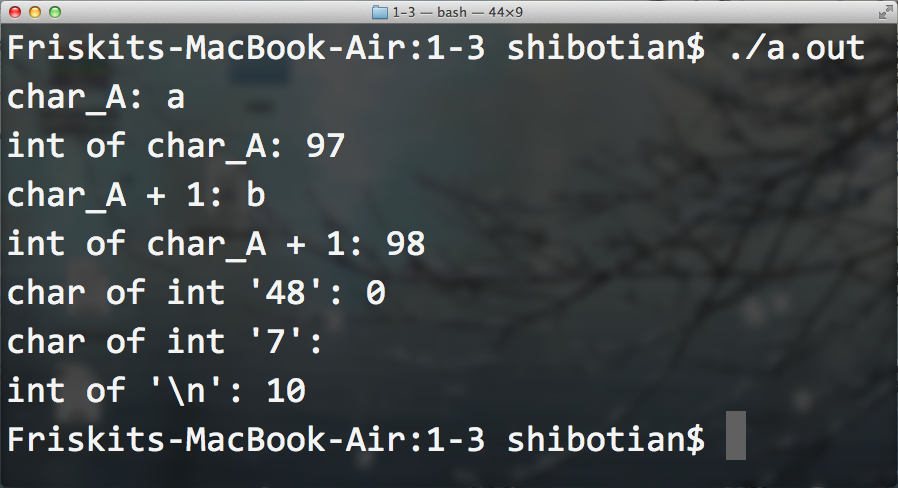
\includegraphics{codes/1-3/result.png}
    \figcaption{字符类型} 
    \label{fig:code-1-3-result} 
  \end{minipage} 
\\[\intextsep] 

在上面的输出中,char\_A的内容是字符‘a’。用强制类型转换的方法可以知道它的“int”值。所以说‘a’的int值是97。然后我们如同对int进行操作一样,对char类型的char\_A进行+1的操作,得到的内容即是数值97+1=98,同时也是ascii码为98的字符‘b’。

后面我们以“char”的方式去输出了一个int类型的“48”。这时候输出结果是“0”。此处的0是打印在屏幕上的字符,而非能够直接计算的数字,因为它在内存中的数据是48。紧接着我们以“char”的方式输出了int类型的“7”。但是屏幕上并未显示任何内容。这是因为在ASCII不但有那些“看得见”的字符(如英文字母、数字),还有很多“看不见”但是有各种功能的字符。例如换行符'$\backslash$n'、制表符等一些控制字符。例如ASCII值为7的字符,实际上是指计算机的蜂鸣器鸣叫一声。大家可以再重新执行一下这段代码,听听是不是有这样的声音。后面又输出了作为换行符的“$\backslash$n”,它的ASCII值为10。

\subsection{Try}

本节内容主要讲解有关字符类型的相关主题,大家可以用前面所学过的知识完成以下的小练习。

\begin{description}
	\item[Try 1]输出一个“可见字符”的ASCII码表。输出字符和其对应的ASCII码。
	\item[Try 2]根据Try 1的结果,找到一种判断给字符分类的方法。分成:大写字母、小写字母、数字、标点符号等。编写一个程序,让用户输入一个字符,屏幕输出这个字符所属的分类。
\end{description}

\section{布尔类型}
布尔是英国的一名数学家,早在18xx年就发明了一系列处理二值运算的逻辑数学方法。所谓二值运算就是“非1即0”。他成功建立了逻辑演算领域,从此,人类可以利用“公式推到”的方法来定量地解决逻辑问题。这一逻辑理论也被人称为布尔代数。

C++中用来表示“二值化”逻辑值的类型就叫做\emph{布尔类型}。布尔类型只有两种取值:true或false,在内存中只占用1字节空间,但由于它只表示两种可能性,所以即便仅用1字节(8位)空间存储,也浪费了八分之七(7位)的空间。但在一些嵌入式设备中对内存管理有着极端的需求,所以可以通过一些位运算的技巧实现1字节存储8个二值化数据。

在这里我们了解一下逻辑运算。逻辑运算不同于算术运算,它的运算符主要是“与”、“或”、“非”。C++中相似的运算一共有两种。一种是普通的“与或非”,另一种则是“位与”、“位或”、“位非”。对于布尔类型而言,由于它在内存中只有最低位表示一个1或者0,所以这两种逻辑运算效果是相同的,但对于那些一般的数值来说,位运算就有自己的神奇之处了!

对于普通的逻辑运算,C++中使用“\&\&”表示与,“||”表示或、“!”表示非。对于这三种运算有如下的真值表:

\begin{center}
	\tabcaption{与运算}
	\label{tab:andOpr}
	\begin{tabular}{|c|c|c|}
		\hline
			$\&\&$	&	$true$	&	$false$	\\
		\hline
			$true$	&	$true$	&	$false$	\\
		\hline
			$false$	&	$false$	&	$false$	\\
		\hline
	\end{tabular}
\end{center}

\begin{center}
	\tabcaption{或运算}
	\label{tab:orOpr}
	\begin{tabular}{|c|c|c|}
		\hline
			$||$	&	$true$	&	$false$	\\
		\hline
			$true$	&	$true$	&	$true$	\\
		\hline
			$false$	&	$true$	&	$false$	\\
		\hline
	\end{tabular}
\end{center}


\begin{center}
	\tabcaption{非运算}
	\label{tab:notOpr}
	\begin{tabular}{|c|c|}
		\hline
					&	$!$		\\
		\hline
			true	&	false	\\
		\hline
			false	&	true	\\
		\hline
	\end{tabular}
\end{center}

从表格中我们可以看出逻辑运算的规则\footnote{与运算在C++中具体的语法规则会在后面的代码中提到}:
\begin{description}
	\item[与运算]两个运算数全为true,结果才为true。只要任何一个是false,则结果就是false。
	\item[或运算]两个运算数只要有一个true,结果就是true。两个全为false是,加过才为false。
	\item[非运算]操作数为true,则结果为false。操作数为false,则结果为true。
\end{description}

而另一种逻辑运算就是“位逻辑运算”。它们的参与运算的不再是操作数整体的布尔值,而是操作数的每一个二进制位。位与运算的运算符是“\&”,位或运算的运算符是“|”,位非运算的运算符是“~”
例如有short a = 385(00000001 10000001)和short b = 128(00000000 10000000)。
\begin{description}
	\item[a\&b] 385 \& 130 = (00000001 10000001) \& (00000000 10000010) = (00000000 10000000) = 128。
	\item[a|b] 385 | 130 = (00000001 10000001) | (00000000 10000010) = (00000001 10000011) = 387
	\item[~a] ~(00000001 10000001) = (11111110 01111110) = -386\footnote{这里的-386和后面的-131都是有符号类型}
	\item[~b] ~(00000000 10000010) = (11111111 01111101) = -131
\end{description}
位逻辑运算就是按照每一个对应位进行的逻辑运算。前面我们曾经说到过用1个字节表示8个不同的逻辑值,就是用位逻辑运算实现的。通过位与0来让某一位置0,通过位或1来让某一位置1。再通过位与1来获得某一位上的值。

既然bool类型也是内存中占用1字节的一种数据类型,在内存中它有256种不同的取值,但对于布尔类型来说只要true和false就足够了。0是false,1是true,那么其他数值呢?
\begin{quote}
	\emph{C++规定,对于bool类型来说,只有0表示false,剩下所有数都表示true}。
\end{quote}

\subsection{Code}

\lstinputlisting[language=C++,caption=布尔类型,label=code:BoolType]{codes/1-4/1-4.cpp}

\subsection{Analyze}

这段代码主要是进行与布尔类型有关的操作,下面是代码中的部分注解:
\showremarks

从代码中我们了解到bool类型可以接受“true”、“false”甚至是数字等等作为值。在代码的第6行可以看到bool\_b被赋值为2,但在第14行输出的时候,发现bool\_b的输出值实际上是1。这是因为在赋值的时候,系统进行“隐含类型转换”——将数字2转换为bool类型的true,而这个true实际上是数字“1”,再将这个1赋值给bool\_b。

而在后面直接输出bool类型时,不难发现,输出的bool类型实际上就是非1即0的数值。这是因为cout会在输出布尔值时自动展开它的整数形式。所以输出的布尔类型的值与将其显示强制类型转换成int之后的值完全一致。

代码的第17、20行,我们测试了对bool类型变量的运算。也不难发现,这样的运算实际上就是对bool类型变量内部的整数值进行的运算。

在代码的24行至28行,程序使用if语句进行不同的操作,可见bool类型能够作为if中进行判断的条件!

在30行以后的代码印证了前面我们见到的位逻辑运算的功能。

\subsection{Result}
代码执行后效果如图:
\\[\intextsep] 
  \begin{minipage}{\textwidth} 
    \centering 
    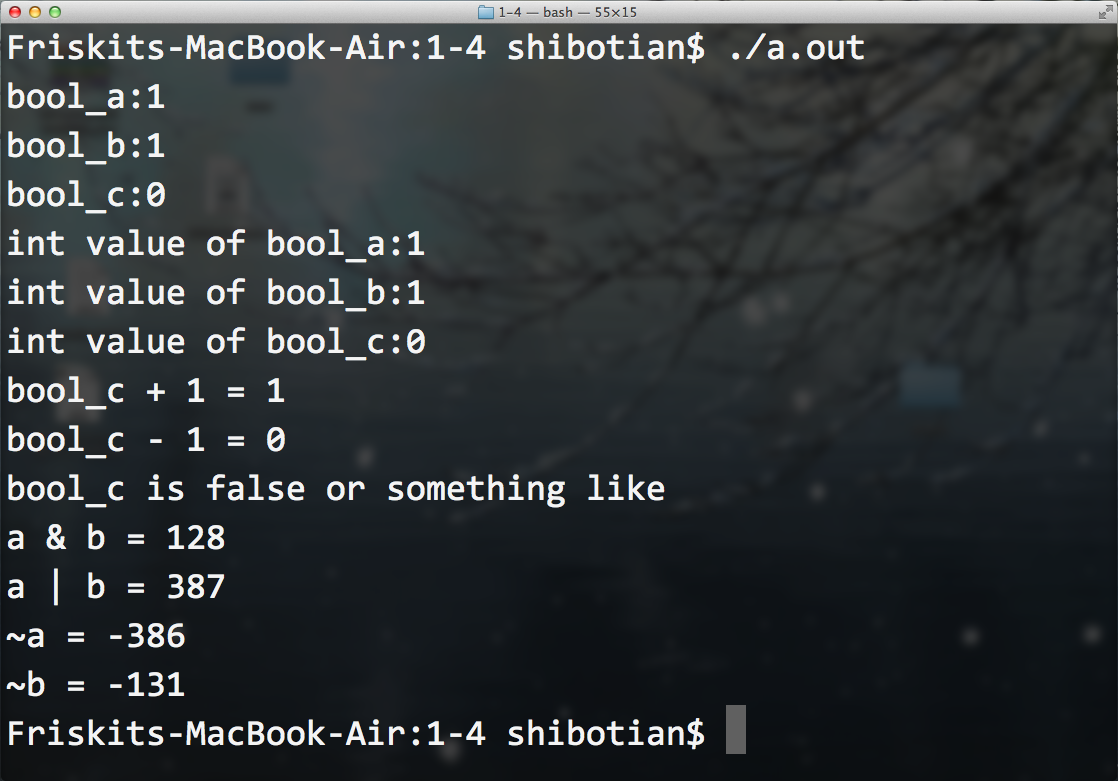
\includegraphics{codes/1-4/result.png}
    \figcaption{布尔类型} 
    \label{fig:code-1-4-result} 
  \end{minipage} 
\\[\intextsep]

在这一节中我们了解到了有关“逻辑运算”的主题。包括了普通的“与或非”和“按位的与或非”。逻辑运算是后面很多内容的基础,在C++中的地位非常重要。位运算代码的字里行间之中充满了小技巧,熟练地使用能够很方便地解决很多复杂的问题!
\subsection{Try}
\begin{description}
	\item[Try 1]用程序验证本节中出现的逻辑运算真值表
	\item[Try 2]实现用一个字节长度的变量存储8个逻辑类型的程序段。依次给每一位赋逻辑值、并依次输出每一位的逻辑值。
\end{description}

\section{运算符与表达式}
其实前面代码的字里行间处处都有表达式的存在。表达式是程序组成的基本部分它们通常是由运算符与操作数组成的式子。由于运算符的种类有很多,而且每种运算符又可以与很多种类型的操作数甚至是表达式组成更加复杂的表达式,所以表达式的种类也有很多。最常见的表达式有“算术表达式”、“赋值表达式”、“关系表达式”、“逻辑表达式”等等。

简单的表达式通常由一个运算符和若干个操作数构成,例如数学中的四则运算、逻辑运算中的与或。它们通常用来描述算法中的最基本的操作。多个简单的表达式能够复合成一个复杂的表达式,用以完成复杂的操作。\emph{任何}一个表达式在运算完成之后都会有一个结果,这个结果包含了某种数据类型的值,称为表达式的值。表达式的值和类型与操作数和运算符的类型有关。

表示内存中某个能够被用户访问的“名字”被称为左值。通常是用户能够读写的变量,并且左值表示的是这个“变量”而不是计算的结果。左值通常出现在赋值符号(等号)的左边,故名左值。左值是一个内存地址,通过左值就可以对该地址下的数据进行处理。与左值对应的则是“右值”。当一个符号或者常量放在赋值符号(等号)右边时,计算机负责读取他们的值,也就是它们所代表的真实值。这个值可能是通过表达式计算而来,也可能是变量、常量等。左值可以看作是“目的地址”,右值相当于“要放入目的地址的数据值”。

在我们的算法中,很少出现只包含两个操作数一个运算符的表达式,更多的是像“int a = $1*2+3/4*(5+6/7)$”。所以说表达式的值不但与表达式内运算符的种类及操作数的类型有关,更与表达式内操作的执行顺序有关。

高级语言都有“隐含”的运算顺序,其中一部分就是数学上的严格规定:例如“先乘除后加减”、“括号最先计算”等等。还有一部分特殊的运算符的特殊的规定:例如“逻辑运算先与后或”等等。这些特殊运算的顺序不再是我们熟悉的顺序,尽管我们可以通过一张详细的“运算符顺序表”来描述清楚,但是我还是建议大家在遇到优先级不明确的运算时一定要用括号进行辅助。因为不论是数学运算还是逻辑运算,“括号内的内容先运算”是亘古不变的道理。

表达式由众多的基本操作组成。常用的操作主要有赋值操作、算数操作、自增操作、关系逻辑操作、条件运算符等多种。涉及包括单目、双目、甚至三目\footnote{所谓“目”就是指操作数的数量,单目运算符就是一个只针对一个操作数进行操作的运算符,例如取反。双目则是操纵两个操作数的运算符,如同数学上的加减乘除等。三目运算符同理。}等多种运算符。其中的一些操作及它们的具体功能会在下面的代码中一一展示!

\subsection{Code}

\lstinputlisting[language=C++,caption=运算符与表达式,label=code:OperatorAndExpression]{codes/1-5/1-5.cpp}

\subsection{Analyze}


在代码\ref{code:OperatorAndExpression}中,罗列了很多有关表达式的操作,下面是代码中的一些注解:
\showremarks

第5行是前面曾经提到过的基本的赋值表达式。等号右边会进行计算,并将最终的计算结果以变量a类型,即int的方式\footnote{如果不是int则转换到int类型}赋值给a。

在后面的几行是几种“复合赋值”表达式。其功能就不再是单一的赋值,而通常是“先进行某种运算,然后再将结果赋值”。例如“+=”就是指“先加后赋值”。“a+=b”就是“a=a+b”。这样的写法不但更加易读\footnote{只是在a的基础上增加一个增量},同时还能提高效率\footnote{因为a会被调用两次。虽然这种情况效率提升不明显,但是当“a”是个复杂的内容(例如函数调用)的时候,它对效率的影响将会非常明显!}。其他诸如此类的还有“-=”、“*=”、“/=”等等非常多的运算符。

代码的第12行进行了一种名为“求模”的运算。其功能是“求余数”。求模运算在日常编程中非常有用!它可以与乘除10配合,用来截取某一位数字。或者用来产生一个“轮回”的效果等等。

从14行开始时自增自减操作,自增自减分为两种:一种是前缀自增自减操作,一种是后缀自增自减操作。这两种操作的区别,大家可以从代码的执行之中推敲出来\footnote{前缀运算是“先运算,后用值”,后缀运算是“先用值后运算”。这里的“后”是指在整个表达式运算完毕之后。例如int a = 0; int b = (a++)+(a++),实际上是b = 0 + 0然后a再经过两次++}。

第28行开始是“关系运算”。所谓关系运算就是指判断两个操作数的关系。常见的有“>”、“<”、“==\footnote{关系运算中判断是否相等是两个等号!!一个等号表示的是赋值符号}”、“!=(不等于)”、“>=”、“<=”等等。关系运算的操作数通常是两个可比较的数,常见的基本数据类型都可以作为它的操作数。比较的结果实际上是bool类型。成立则是1,不成立则是0。

第35行开始是“逻辑运算”。在前面的章节我们已经提到过,逻辑运算就是将“逻辑值”作为操作数的一种运算。逻辑运算主要包括“与——\&\&”、“或——||”、“非——!”

第47行开始介绍了“左运算符('<<')和右运算符('>>')”。这两种运算符是C++中附带的运算符,具体的功能会根据操作数的不同而有所不同。我们也可以根据需要来实现自定义的功能。例子中的运算符的功能是“位移”。“a>>b”就是指将a的二进制位右移b位,“<<”则表示左移。

程序的最后(56行)是一个复杂表达式的例子。在这个例子中大家可以看到很多操作其实都是可以放在同一个表达式中执行的。程序首先执行“\_a==\_b”返回值是true,再对其取反则为false,所以\_c的值应为冒号右边的“true”。面对这种复杂的表达式,应该从运算优先级入手,先计算优先级最高的部分(通常用小括号括起来)。然后再逐层计算得到结果。

\subsection{Result}
代码执行后的输出结果如图:
\\[\intextsep] 
  \begin{minipage}{\textwidth} 
    \centering 
    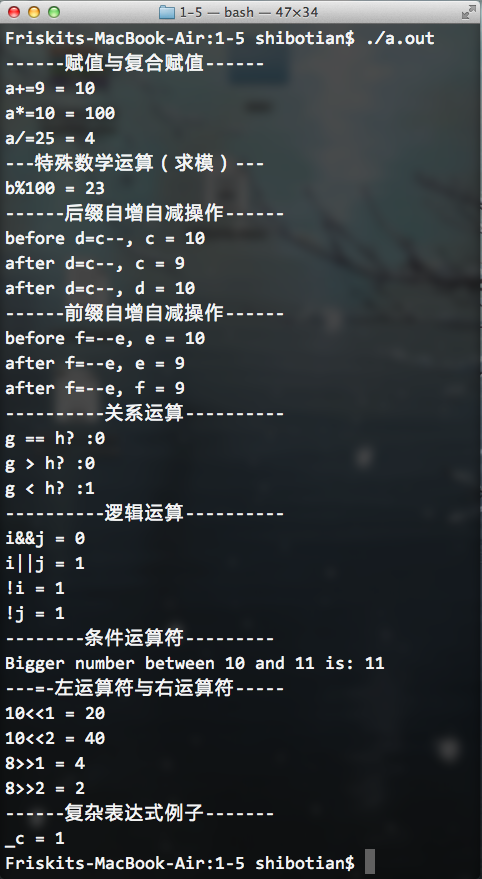
\includegraphics{codes/1-5/result.png}
    \figcaption{运算符与表达式} 
    \label{fig:code-1-5-result} 
  \end{minipage} 
\\[\intextsep]

本节的内容是表达式与运算符。学到这里,你应该已经了解到各种运算符在C++中的使用方法了。

\subsection{Try}
\begin{description}
	\item[Try 1]用程序运算$\frac{((2\times3)+4)}{2}\times0.5$的结果
	\item[Try 2]编写一个程序,提示用户输入半径r,并且计算以r为半径的圆的面积和周长,($\pi=3.14$)
	\item[Try 3]编写一个程序,让用户输入一个5位数,然后将这五位数的反过来输出,例如输入12345,输出54321.(提示,利用求模和除法)
\end{description}

\section{语句与控制}
语句是构成程序的基本单元,通常由简单的语句表示一个简单的动作、或者由复合语句来表示一组复杂的操作。
语句是由按照一定语法规则排列的单词组成,单词之间由运算符、分隔符或空格分割。在C++中的语句以分号作为结束的标志。之所以使用一个分号分割语句,是因为C++编译器通常不将“换行”等操作看作是分割语句的标志,甚至我们也可以将多个语句由分号分割后写在同一行。
在C++中主要包含四种语句类型:

\begin{enumerate}
	\item{表达式语句}
	\item{复合语句}
	\item{选择语句}
	\item{循环语句}
\end{enumerate}

表达式语句的构成非常简单,就是任何表达式结尾处跟着一个语句的标志——分号“;”即可。这样就构成了表达式语句。

复合语句的构成也非常简单。通常来说,一个语句难以完成一系列功能,所以我们把多条表达式语句顺序写成,然后放在两个大括号之中,事就这么成了。复合语句将很多条语句看成是一个不可分割的整体。利用大括号将独立功能的一块括起来,这是一种很好的编程风格,但其实这种用法更多见于后面介绍的各种控制语句之中。

一般来说,在程序中语句逐行罗列,程序也依次执行。这一种上下两条语句紧密相连的结构被成为“顺序结构”。除此之外,我们在前面的小节中也遇到过“当A则B否则C”的执行方式。这种方式由一个条件去控制究竟是B被执行,还是C被执行?这种结构我们称为“选择结构”。除此之外,当我们要重复处理大量近似的操作时,使用顺序结构是非常麻烦的,所以这时候就有了“循环结构”。利用循环结构,我们可以用简洁的描述实现复杂的功能。这些算法中的抽象的控制结构,在C++中使用“选择语句”、“循环语句”来体现\footnote{顺序语句在哪里?其实除了这两种结构以外我们所逐行书写的代码都属于顺序语句。}。在这几种控制语句之中,还穿插着诸如“break”、“continue”等特殊的语句用来进行一些“精巧”的控制。

上面所述的语句概念颇多,我将在接下来的Code部分为大家举例说明。

\subsection{Code}

\lstinputlisting[language=C++,caption=语句,label=code:Statement]{codes/1-6/1-6.cpp}

\subsection{Analyze}
这段代码中出现了“选择语句”、“循环语句”以及一些直接控制语句(break、continue)等语句,下面是代码中的注解:
\showremarks

代码第7-15行展示了“条件语句”的使用。条件语句的形式主要是:

\begin{lstlisting}[xleftmargin=10em,xrightmargin=10em]
if(<布尔表达式A>)
    <语句A>
else
    <语句B>
\end{lstlisting}

这段代码是非常简单的if语句的形式,甚至我们在前面已经见过。其中布尔表达式应该是一个能返回布尔值或者等同作用的表达式。例如返回true、false、0、1、10等等。当某个表达式成立,则跟他相配得那部分代码会被执行。如果仅仅是一个if不够,还可以用多个else if。语句中可以是单条语句,也可以是用大括号括起来的复合语句。,如同这样:

\begin{lstlisting}[xleftmargin=6em,xrightmargin=6em]
if(<布尔表达式A>)
    <语句块A>
else{
    if(<布尔表达式B>)
        <语句块B>
    else{
        if(<布尔表达式C>)
            <语句块C>
        else{
            ...
                ...
        }
    }
}
\end{lstlisting}

上面这样的嵌套if语句执行流程如图:

\begin{center}
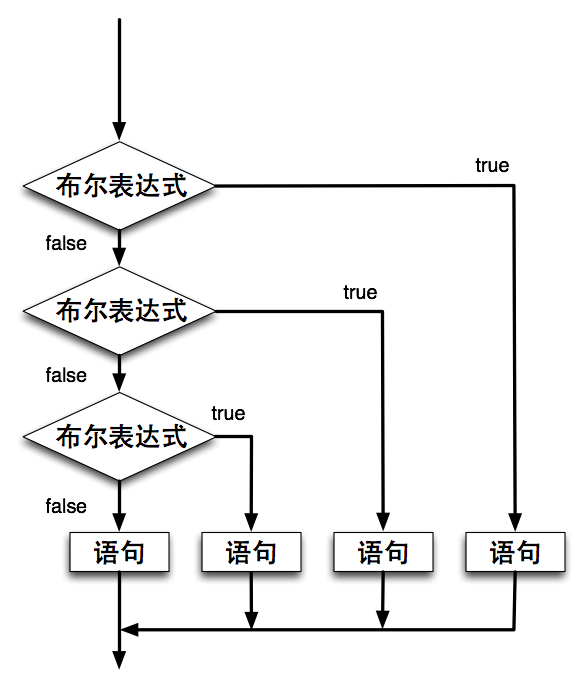
\includegraphics{fig/1-6/1_if_statement.png}
\end{center}

不难发现,这种写法非常复杂和臃肿,我们可以用下面的方法完全等效地代替:

\begin{lstlisting}[xleftmargin=10em,xrightmargin=10em]
if(<布尔表达式A>)
    <语句块A>
else if(<布尔表达式B>)
    <语句块B>
else if(<布尔表达式C>)
    <语句块C>
...
	...
else
    <语句块Z>
\end{lstlisting}

上面的例子已经告诉我们,if语句的语句块中也是语句,也就是说可以再嵌套插入其他诸如循环、选择等语句。但要注意,当嵌套使用if语句时可能会产生括号匹配的问题。例如:

\begin{lstlisting}[xleftmargin=10em,xrightmargin=10em]
if(<布尔表达式A>)
    if(<布尔表达式B>)
        <语句块B>
else
    <语句块C>
\end{lstlisting}

在上面代码之中,出现了两个嵌套的if语句。如果语句块B和C中的内容都是没有大括号包围的单条语句,那么第4行的else究竟应该与哪个相匹配?在C++中规定,else跟在它上面与它最近的else相匹配。这个特性能够消除嵌套使用if语句的二义性。也就是说,即便根据缩进看起来第四行的else与第一行的if相配,但实际上它会去寻找上面离它最近的也就是第2行的if语句。

这种二义性是由于使用“单条语句”而非“语句块”而导致的。所以作为初学者,如果还是不太习惯这条规则,可以将if语句中的语句块都用大括号括起来,形成“复合语句”。

代码\ref{code:Statement}的第18行,出现了一个switch语句。这个语句又叫做“开关语句”。开关语句会寻找到一个入口,然后将入口以后的程序依次执行,直到执行完毕或者遇到break。开关语句的形式是这样的:

\begin{lstlisting}[xleftmargin=10em,xrightmargin=10em]
switch(<整型表达式>){
    case <整型常量表达式A>:
        <语句A>
    case <整型常量表达式B>:
        <语句B>
    ...
        ...
    default:
        <语句Z>
}
\end{lstlisting}

我们曾在上面看到过连续的else-if语句,开关语句只是它的一种精简版。<整形表达式>将会被运算并且得到值,紧接着程序就会在后面的一组case的<整型常量表达式>中找到一个与之相等的常量。以此case作为入口,从该语句处连续执行,直到遇到break或者switch语句执行完毕。

当在case的<整型常量表达式>中找不到相匹配的常量,则程序会以default作为入口。dafult是可以省略的,它的位置也是可以调换的。但倘若default出现在switch里的第一行,则后面的case也就失去意义,因为程序第一个找到的入口就是default。

在代码\ref{code:Statement}的38行,介绍了一种循环语句——while语句。while语句的形式如:
\begin{lstlisting}[xleftmargin=10em,xrightmargin=10em]
while(<表达式>)
    <语句>
\end{lstlisting}

其中的语句可以是单条语句、也可以是复合语句块。程序执行的流程是:计算表达式的值,如果为true则会执行语句,然后再次计算表达式的值,如果为真则执行语句....直到执行表达式时值为假,则跳出while循环。用图示来说明就是这个样子:

\begin{center}
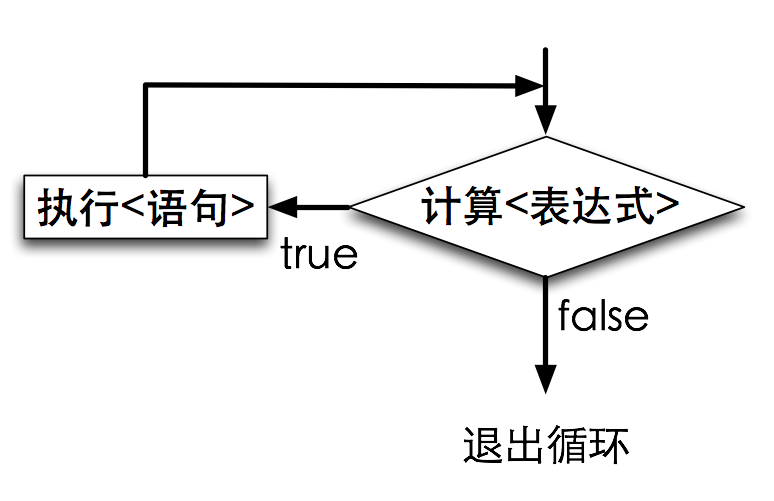
\includegraphics{fig/1-6/2_while_statement.png}
\end{center}

在while循环中,我们通过括号内的表达式控制循环的进入。通常在循环之中要修改一些能够使表达式取值不同的值。只有表达式的值从true变为false,才能退出循环,否则程序将进入无休止的死循环。while比较适合循环次数无法预知的循环。

除此之外在代码\ref{code:Statement}的第45行还出现了另一种形式的while循环——do-while循环。通常的while循环需要先计算表达式的值,再判断是否能进入循环。循环内的语句可能一次都不会被执行\footnote{因为第一次执行循环表达式时结果就为false}。当我们想要至少要让循环内容执行一次再进行判断,那么就需要用do-while循环了。

do-while循环的形式如下:

\begin{lstlisting}[xleftmargin=10em,xrightmargin=10em]
do
    <语句>
while(<表达式>);
\end{lstlisting}

它的执行流程与while类似,只不过do后面的<语句>会被先执行一次,然后再由<表达式>的值判断下次是否要进入循环。它的执行流程如图:

\begin{center}
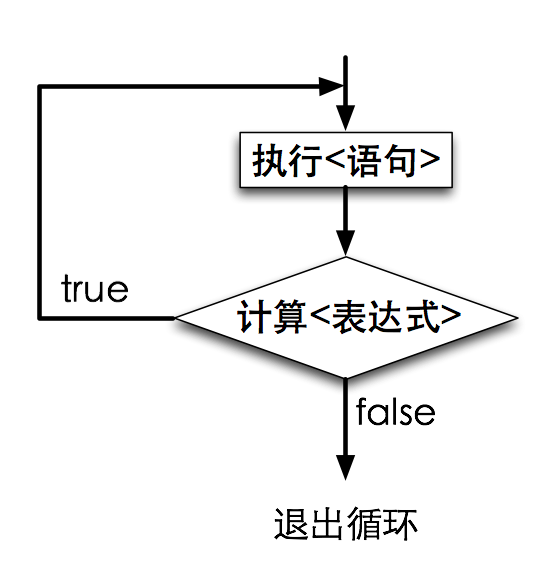
\includegraphics{fig/1-6/3_dowhile_statement.png}
\end{center}

代码\ref{code:Statement}的第52行,出现了另外一种循环语句——for循环。for循环实际上是一串复杂操作的集合体。for循环的形式如下:

\begin{lstlisting}[xleftmargin=6em,xrightmargin=6em]
for(<表达式A>;<表达式B>;<表达式C>)
    <语句>
\end{lstlisting}

for循环的风格比较适用于\footnote{“适用于”不代表不能用于其他情况。但是这些都属于编程技巧的范畴,本章不过多阐释。}直观地描述循环次数可以预知的确定性的循环。在<表达式A>,<表达式B>,<表达式C>中,\emph{通常}都会包含用户定义的一个变量,该变量成为“循环变量”或“索引变量”。循环变量的定义和赋初值通常在<表达式A>中进行。<表达式B>的取值将决定这个for循环进行与否,如果该值为true,则循环继续,为false则终止。在这里通常让循环变量与一个“界”相比较。这个界能够很好地控制循环次数。<表达式C>则用来对循环变量进行修改,使得<表达式B>中的值能够产生变化。通常在这里给循环变量一个某步长的增量,用以控制循环。<语句>中的内容则成为是循环体。可以使任何类型的可执行语句,可以是包括多条语句的复合语句,甚至可以是空语句\footnote{这种没有循环体的循环可以在一些程序中用来延时、或者仅使用循环中三个表达式就能完成一些操作}。for循环复杂的执行流程可以用下图简单地表示:

\begin{center}
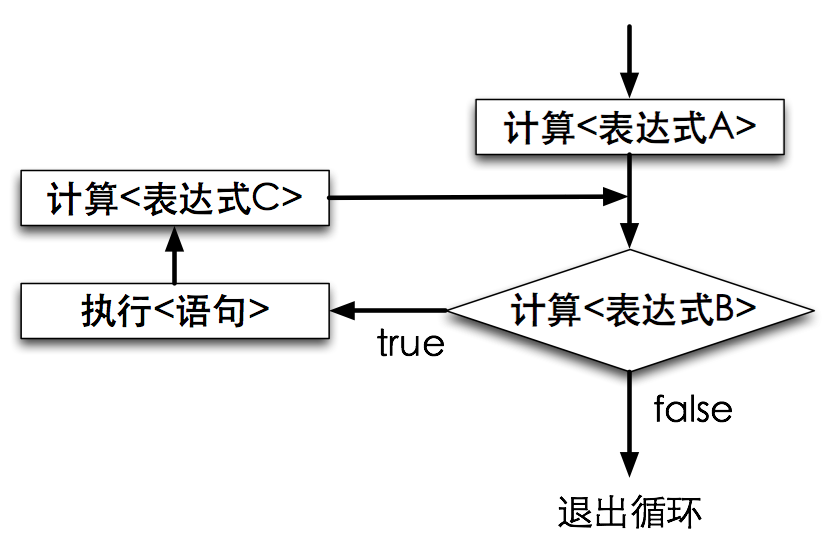
\includegraphics{fig/1-6/4_for_statement.png}
\end{center}

程序首先执行一次<表达式A>,由于它只会被执行一次的特性,所以通常用来初始化变量。然后进入一个类似while循环的结构,以<表达式B>作为循环控制,不断地执行<语句>并重新计算<表达式C>。知道<表达式B>的值不在满足,则跳出循环。

代码\ref{code:Statement}第58处开始的for循环中,使用了break和continue语句。break的作用是立即跳出当前的循环,开始执行循环之后的内容。而continue的功能是跳过本次循环体内语句的执行,但循环体外(<表达式C>)不受影响,还是会执行。

\subsection{Result}
让我们看看上面代码执行之后的结果吧:
\\[\intextsep] 
  \begin{minipage}{\textwidth} 
    \centering 
    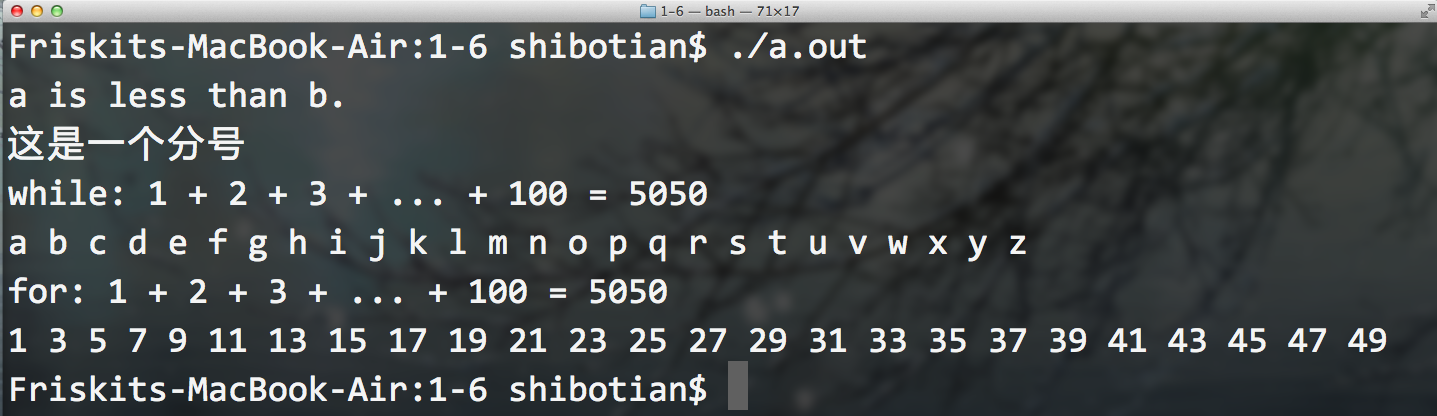
\includegraphics{codes/1-6/result.png}
    \figcaption{语句} 
    \label{fig:code-1-6-result} 
  \end{minipage}
\\[\intextsep]

程序首先进入if语句,由于a=10<11,所以会输出“a is less than b”。其他并列的几个else将不会进入。

在后面的switch中,程序判断变量c中的内容。当程序发现c的内容与第28行的分号匹配,所以程序的入口是第29行。输出“这是一个分号”,然后在break的作用下跳出整个switch语句。

在第38行,程序使用while循环进行1至100的求和运算。使用变量d作为控制变量和计数器,sum\_d每次在原有基础上增加d,同时使d自加。当d达到100时跳出循环并输出结果。

在第45行,程序使用do-whiel语句输出了从a到z的26个字母,每次变量e+1,其ascii对应的字母就会增长一个。

紧接着第52行是使用for循环进行1至100求和。其实现功能与while循环所实现的完全一致,但写法各有差异。

第58行的for循环中使用了break和continue。程序首先定义i=1,并且发现控制条件为true,程序会进入循环,判断当i=50时跳出循环\footnote{使用这种方法控制循环次数非常简陋,此处只为作为例子,请大家不要学习这种风格},此时整个循环过程结束,否则继续执行。程序又判断i是否是偶数如果是偶数则执行continue语句,跳过本次循环体的剩余内容,也就是不执行第63行的输入。如果前面两个if都不满足,则说明i此时一定是一个小于50的奇数,并将它输出。

在本节中,我们主要介绍了语句的概念。平时我们以此编写的语句罗列在一起就是顺序结构,除此之外还可以有选择结构和循环结构。在这几种结构的帮衬下,我们至此可以实现很多很多有趣的算法。

\subsection{Try}
本节内容比较多,所以Try中的内容也会比较多,希望大家能够看清每一个要求、认真编写好每一段程序。
\begin{description}
	\item[Try 1]编写一个问候程序,由用户输入当前小时(24)时制。输出问候语(如早上好、中午好等)。让这个程序直到关闭之前能够不断运行。
	\item[Try 2]统计不同种类字符的字数:让用户不断输入内容(直到输入#号终止),并且统计用户曾经输入不同类型字符(数字、小写字母、大写字母、其他符号)的个数。
	\item[Try 3]编写一个程序,让用户输入一个数n,求从1到n之间所有整数求和。
	\item[Try 4]编写程序输出一个由“*”组成的,长10,宽20的矩形。
	\item[Try 5]代码:“for(int i=0;i<10;i++)cout<<'!'<<endl;”其中一共会输出多少个“!”?
	\item[Try 6]使用循环计算斐波那契数列的第20项。(斐波那契数列是指f(n)=f(n-1)+f(n-2),即从第三项起,每项值是其前两项和,第一项和第二项是1。)
	\item[Try 7]编写一个5分制打分系统。根据用户的得分输出相应等级。例如输入5分,输出:优秀;输入0分,输出“非常差”。
	\item[Try 8]找到1-100000中所有3的倍数。并且统计这些数有几个。
\end{description}

